\documentclass[sigconf]{acmart}

\usepackage{algorithmic}
\usepackage{algorithm}
\usepackage{hyperref}
\usepackage[newfloat,cache=false]{minted}

\begin{document}

\title{Lab 2 Exercise - PyTorch Autograd}
\author{Luke McClure}
\email{29573904}

\maketitle
\pagestyle{myheadings}
\section{Exercise 1}
\subsection{Implement gradient-based factorisation using PyTorch's AD}
\begin{listing}[H]
    \begin{minted}[frame=lines, breaklines, breaksymbolleft=, fontsize=\footnotesize]{python}
def sgd_factorise_ad(A: torch.Tensor, rank: int, num_epochs = 1000, lr = 0.01):
    m = A.shape[0]
    n = A.shape[1]
    U = torch.rand(m, rank, dtype=A.dtype, requires_grad=True)
    V = torch.rand(n, rank, dtype=A.dtype, requires_grad=True)

    for epoch in range(num_epochs):
        #reset grad
        U.grad = None
        V.grad = None

        #calc error and grad
        e = torch.nn.functional.mse_loss(A, U @ V.t(), reduction='sum')
        e.backward()

        #update using grad
        with torch.no_grad():
            U -= lr * U.grad
            V -= lr * V.grad
    return [U, V]
    \end{minted}
\end{listing}
\subsection{Factorise and compute reconstruction error on real data} 
\begin{center}
    \begin{tabular}{| c c |}
        \hline
        Algorithm & Loss \\ 
        \hline\hline
        sgd\_factorise\_ad & 15.2 \\
        truncated SVD & 15.2\\
        \hline      
    \end{tabular}
\end{center}
The reconstruction loss between sgd\_factorise\_ad and truncated SVD are almost exactly the same. The gradient descent method of reconstruction is able to capture all the reconstruction properties of the analytical method of svd. 
\subsection{Compare against PCA}
The data projected on to the first two principal components is roughly equivalent to the scatter plot of the first two columns of U.
By performing a linear transform (specifically avertical, horizontal, then vertical flip) the two plots are identical in all but a few degrees of orientation.

In order to accurately reconstruct data (ie minimise reconstruction error) it is important to capture the variance of the data along several axis. This feature is also crucial in transforming data into lower dimensional space in the way PCA does, as a result the two are very similar processes.

\begin{figure}[H]
    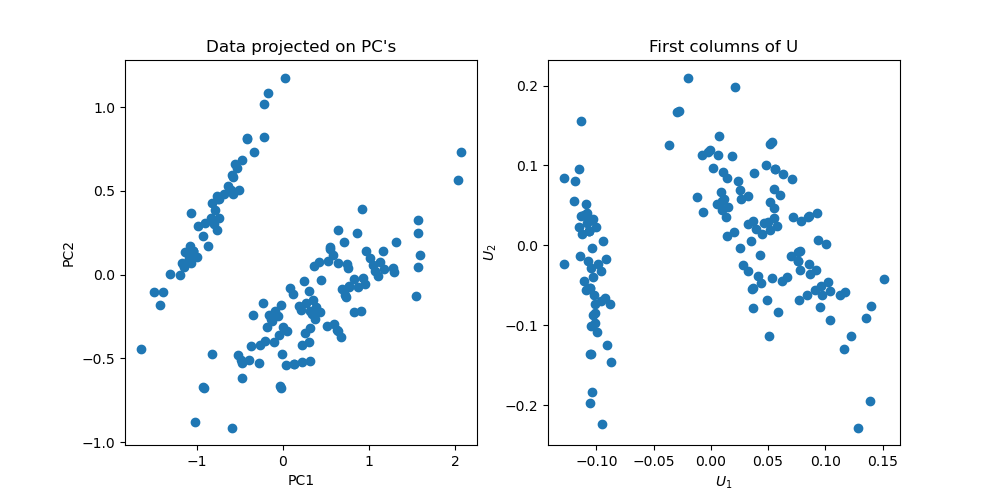
\includegraphics[width=\linewidth]{../pcacomparison.png}
\end{figure}

\section{Exercise 2}
\subsection{Implement the MLP}
\begin{listing}[H]
    \begin{minted}[frame=lines, breaklines, breaksymbolleft=, fontsize=\footnotesize]{python}
def MLP_train(data: torch.Tensor, targets: torch.Tensor, num_epochs = 100, lr = 0.01):
    W1 = torch.randn(4, 12, requires_grad=True)
    W2 = torch.randn(12, 3, requires_grad=True)
    b1 = torch.tensor(0.0, requires_grad=True)
    b2 = torch.tensor(0.0, requires_grad=True)

    for epoch in range(num_epochs):
        #reset grad
        W1.grad = None
        W2.grad = None
        b1.grad = None
        b2.grad = None

        #calc weight and grad
        logits = torch.relu(data @ W1 + b1) @ W2 + b2
        loss = torch.nn.functional.cross_entropy(logits, targets)
        loss.backward()

        #update using grad
        W1.data = W1 - lr * W1.grad
        W2.data = W2 - lr * W2.grad
        b1.data = b1 - lr * b1.grad
        b2.data = b2 - lr * b2.grad

    loss = torch.nn.functional.cross_entropy(logits, targets).item()
    return [[W1, b1], [W2,b2], loss]      
    \end{minted}
\end{listing}
\subsection{Test the MLP}
\begin{center}
    \begin{tabular}{| c c c|}
        \hline
        Run & Training Loss & Validation Loss\\ 
        \hline\hline
        1 & 0.4293 & 0.4288 \\
        2 & 0.3914 & 0.5668 \\
        3 & 0.4314 & 0.3880\\
        4 & 0.4271 & 0.5501\\
        5 & 0.6610 & 0.7730\\
        \hline\hline
        Mean & 0.4680 & 0.5413\\
        \hline      
    \end{tabular}
\end{center}
The validation loss is usually slightly higher than the training loss as the MLP is able to adapt to losses within the training set, the validation set is completely unseen to it.
In some cases the validation loss is lower than training, if the model is well generalised training and validation loss should be roughly equal.
\end{document}
\endinput